% This is text associated with the open textbook "Open Electromagnetics"
% See immediately below for author, date
% This work is licensed under the Creative Commons Attribution-ShareAlike 4.0 International License. (CC BY SA 4.0) 
% To view a copy of the license, visit http://creativecommons.org/licenses/by-sa/4.0/

%ORB TITLE Magnetic Force on a Current-Carrying Wire
%ORB AUTHOR 0        # S.W. Ellingson, Virginia Tech (ellingson@vt.edu)
%ORB DATE 20191117   # yyyymmdd
%ORB ABSTRACT 

\label{m0017_Magnetic_Force_Current-Carrying_Wire} % <-- Must match name of this file and module directory name.  Don't mess with this!

Consider an infinitesimally-thin and perfectly-conducting wire bearing a current $I$ (SI base units of A) in free space.  
Let ${\bf B}\left({\bf r}\right)$ be the impressed magnetic flux density at each point ${\bf r}$ in the region of space occupied by the wire.
By \emph{impressed}, we mean that the field exists in the absence of the current-carrying wire, as opposed to the field that is induced by this current.
Since current consists of charged particles in motion, we expect that ${\bf B}({\bf r})$ will exert a force on the current. 
Since the current is constrained to flow on the wire, we expect this force will also be experienced by the wire.
Let us now consider this force.

To begin, recall that the force exerted on a particle bearing charge $q$ having velocity ${\bf v}$ is
%
\begin{equation}
{\bf F}_m\left({\bf r}\right) = q{\bf v}\left({\bf r}\right) \times {\bf B}\left({\bf r}\right) 
\end{equation}
%
Thus, the force exerted on a \emph{differential} amount of charge $dq$ is
%
\begin{equation}
d{\bf F}_m\left({\bf r}\right) = dq~{\bf v}\left({\bf r}\right) \times {\bf B}\left({\bf r}\right) 
\end{equation}
%
Let $d{\bf l}\left({\bf r}\right)$ represent a differential-length segment of the wire at ${\bf r}$, pointing in the direction of current flow.
Then 
%
\begin{equation}
dq~{\bf v}\left({\bf r}\right) = I d{\bf l}\left({\bf r}\right)
\end{equation}
%
(If this is not clear, it might help to consider the units:
On the left, C$\cdot$m/s $=$ (C/s)$\cdot$m $=$ A$\cdot$m, as on the right.)
Subsequently,
\begin{equation} 
d{\bf F}_m\left({\bf r}\right) = I d{\bf l}\left({\bf r}\right) \times {\bf B}\left({\bf r}\right) 
\label{m0017_edmforce}
\end{equation} 

There are three important cases of practical interest.  
First, consider a straight segment ${\bf l}$ forming part of a closed loop of current in a spatially-uniform impressed magnetic flux density ${\bf B}\left({\bf r}\right)={\bf B}_0$.
In this case, the force exerted by the magnetic field on such a segment is given by Equation~\ref{m0017_edmforce} with $d{\bf l}$ replaced by ${\bf l}$; i.e.: 
%
\begin{equation} 
\boxed{
{\bf F}_m = I {\bf l} \times {\bf B}_0 
}
\label{m0017_emforce}
\end{equation} 
%
Summarizing, 
%%%%%%%%%%%%%%%%%%%%%%%%%%%%%%%%%%%%%%%%%%%%%%%
%ORB HIGHLIGHT
\begin{mdframed}[backgroundcolor=yellow!20,nobreak=true] 
The force experienced by a straight segment of current-carrying wire in a spatially-uniform magnetic field is given by Equation~\ref{m0017_emforce}.
\end{mdframed}
%%%%%%%%%%%%%%%%%%%%%%%%%%%%%%%%%%%%%%%%%%%%%%% 

The second case of practical interest is a rigid closed loop of current in a spatially-uniform magnetic flux density 
${\bf B}_0$.  
If the loop consists of straight sides -- e.g., a rectangular loop -- then the force applied to the loop is the sum of the forces applied to each side separately, as determined by Equation~\ref{m0017_emforce}.
However, we wish to consider loops of arbitrary shape.
To accommodate arbitrarily-shaped loops, let $\mathcal{C}$ be the path through space occupied by the loop.  Then the force experienced by the loop is
%
\begin{flalign}
{\bf F} &= \int_{\mathcal{C}} d{\bf F}_m\left({\bf r}\right) \nonumber \\
        &= \int_{\mathcal{C}} I d{\bf l}\left({\bf r}\right) \times {\bf B}_0   
\end{flalign}
%
Since $I$ and ${\bf B}_0$ are constants, they may be extracted from the integral:
%
\begin{equation}
{\bf F} = I \left[ \int_{\mathcal{C}} d{\bf l}\left({\bf r}\right) \right] \times {\bf B}_0  
\end{equation}
%
Note the quantity in square brackets is zero. Therefore: 
%
%ORB HIGHLIGHT
\begin{mdframed}[backgroundcolor=yellow!20,nobreak=true] 
The net force on a current-carrying loop of wire in a uniform magnetic field is zero. 
\end{mdframed}
%
Note that this does not preclude the possibility that the rigid loop \emph{rotates}; for example, the force on opposite sides of the loop may be equal and opposite.  What we have found is merely that the force will not lead to a \emph{translational} net force on the loop; e.g., force that would propel the loop away from its current position in space. The possibility of rotation without translation leads to the most rudimentary concept for an electric motor.  
\index{motor}
Practical electric motors use variations on essentially this same idea; see ``Additional Reading'' for more information.

The third case of practical interest is the force experienced by two parallel infinitesimally-thin wires in free space, as shown in Figure~\ref{m0017_f2wires}.
Here the wires are infinite in length (we'll return to that in a moment), lie in the $x=0$ plane, are separated by distance $d$, and carry currents $I_1$ and $I_2$, respectively.
The current in wire~1 gives rise to a magnetic flux density ${\bf B}_1$.
The force exerted on wire~2 by ${\bf B}_1$ is:
%
\begin{equation} 
{\bf F}_2 = \int_{\mathcal{C}} \left[ I_2 d{\bf l}\left({\bf r}\right) \times {\bf B}_1\left({\bf r}\right) \right]
\label{m0017_eF2}
\end{equation}
%
where $\mathcal{C}$ is the path followed by $I_2$, and $d{\bf l}\left({\bf r}\right)=\hat{\bf z}dz$.  
A simple way to determine ${\bf B}_1$ in this situation is as follows.  
First, if wire~1 had been aligned along the $x=y=0$ line, then the magnetic flux density everywhere would be
%
$$ \hat{\bf \phi}\frac{\mu_0 I_1}{2\pi\rho} $$
%
In the present problem, wire~1 is displaced by $d/2$ in the $-\hat{\bf y}$ direction.  
Although this would seem to make the new expression more complicated, note that the only positions where values of ${\bf B}_1\left({\bf r}\right)$ are required are those corresponding to $\mathcal{C}$; i.e., points on wire~2.  For these points,
%
\begin{equation}
{\bf B}_1\left({\bf r}\right) = -\hat{\bf x}\frac{\mu_0 I_1}{2\pi d} ~~~ \mbox{along}~\mathcal{C} 
\end{equation}
%
That is, the relevant distance is $d$ (not $\rho$), and the direction of ${\bf B}_1\left({\bf r}\right)$ for points along $\mathcal{C}$ is $-\hat{\bf x}$ (not $\hat{\bf \phi}$).
Returning to Equation~\ref{m0017_eF2}, we obtain:
%
\begin{flalign} 
{\bf F}_2 &= \int_{\mathcal{C}} \left[ I_2~\hat{\bf z}dz \times \left(-\hat{\bf x}\frac{\mu_0 I_1}{2\pi d}\right) \right] \nonumber \\
          &= -\hat{\bf y}\frac{\mu_0 I_1 I_2}{2\pi d} ~ \int_{\mathcal{C}} dz
\end{flalign}
%
The remaining integral is simply the length of wire~2 that we wish to consider.
Infinitely-long wires will therefore result in infinite force. 
This is not a very interesting or useful result.
However, the force \emph{per unit length} of wire is finite, and is obtained simply by dropping the integral in the previous equation.
We obtain:
%
\begin{equation}
\frac{{\bf F}_2}{\Delta l} = -\hat{\bf y}\frac{\mu_0 I_1 I_2}{2\pi d} 
\end{equation}
%
where $\Delta l$ is the length of the section of wire~2 being considered.
Note that when the currents $I_1$ and $I_2$ flow in the same direction (i.e., have the same sign), the magnetic force exerted by the current on wire~1 pulls wire~2 toward wire~1.
%
\begin{figure}[b!]
\begin{center}
\pdftooltip{{  % note double braces
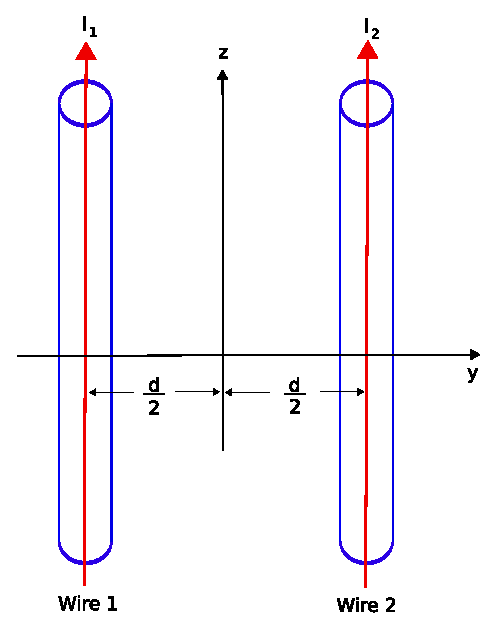
\includegraphics[width=0.8\columnwidth]{modules/m0017_f2wires.eps} 
}}{A y-z coordinate system with wires 1 and 2 parallel. They are equidistant on either side of z-axis from the bottom to the top of the diagram. Current flowing in same direction for both from bottom to top. Wire 1 has current labeled I subscript 1 and wire 2 has current labeled I subscript 2. Wire 1 is distance d over 2 from the z axis on the left and wire 2 is distance d over 2 from the z axis on the right.}
\end{center}
\centerline{\scriptsize 
\copyright~\hyperref[m0017_f2wires_Credit]{Y.\ Zhao} 
\href{https://creativecommons.org/licenses/by-sa/4.0/}{CC BY-SA 4.0} 
} 
\caption{
\label{m0017_f2wires}
Parallel current-carrying wires.
}
\end{figure}

The same process can be used to determine the magnetic force ${\bf F}_1$ exerted by the current in wire~1 on wire~2. 
The result is
%
\begin{equation}
\frac{{\bf F}_1}{\Delta l} = +\hat{\bf y}\frac{\mu_0 I_1 I_2}{2\pi d} 
\end{equation}
%
When the currents $I_1$ and $I_2$ flow in the same direction (i.e., when the product $I_1 I_2$ is positive), then the magnetic force exerted by the current on wire~2 pulls wire~1 toward wire~2.  

We are now able to summarize the results as follows: 
%%%%%%%%%%%%%%%%%%%%%%%%%%%%%%%%%%%%%%%%%%%%%%%
%ORB HIGHLIGHT
\begin{mdframed}[backgroundcolor=yellow!20,nobreak=true] 
If currents in parallel wires flow in the same direction, then the wires attract; whereas if the currents flow in opposite directions, then the wires repel.
\end{mdframed}
%%%%%%%%%%%%%%%%%%%%%%%%%%%%%%%%%%%%%%%%%%%%%%%
Also:
%%%%%%%%%%%%%%%%%%%%%%%%%%%%%%%%%%%%%%%%%%%%%%%
%ORB HIGHLIGHT
\begin{mdframed}[backgroundcolor=yellow!20,nobreak=true] 
The magnitude of the associated force is $\mu_0 I_1 I_2/2\pi d$ for wires separated by distance $d$ in non-magnetic media.
\end{mdframed}
%%%%%%%%%%%%%%%%%%%%%%%%%%%%%%%%%%%%%%%%%%%%%%%

If the wires are fixed in position and not able to move, these forces represent stored (potential) energy.  
It is worth noting that this is precisely the energy which is stored by an inductor -- for example, the two wire segments here might be interpreted as segments in adjacent windings of a coil-shaped inductor.

%%%%%%%%%%%%%%%%%%%%%%%%%%%%%%%%%%%%%%%%%%%%%%%
%ORB EXAMPLE
~\\ \begin{example} 
\begin{mdframed}[backgroundcolor=brown!20,linecolor=brown!20]\raggedright
DC power cable. 
\\~\\
A power cable connects a 12~V battery to a load exhibiting an impedance of $10~\Omega$.
The conductors are separated by 3~mm by a plastic insulating jacket.
Estimate the force between the conductors.

{\bf Solution.}
The current flowing in each conductor is 12~V divided by $10~\Omega$, which is 1.2~A.  
In terms of the theory developed in this section, a current $I_1=+1.2$~A flows from the positive terminal of the battery to the load on one conductor, and a current $I_2=-1.2$~A returns to the battery on the other conductor. 
The change in sign indicates that the currents at any given distance from the battery are flowing in opposite directions.
Also from the problem statement, $d=3$~mm and the insulator is presumably non-magnetic.
Assuming the conductors are approximately straight, the force between conductors is
$$ \approx \frac{\mu_0 I_1 I_2}{2\pi d} \cong -96.0~\mu\mbox{N} $$
with the negative sign indicating that the wires repel.
\end{mdframed}
% note figures will need to go between "\end{mdframed}" and "\end{example}"
\end{example}
%%%%%%%%%%%%%%%%%%%%%%%%%%%%%%%%%%%%%%%%%%%%%%%

Note in the above example that this force is quite small, which explains why it is not always observed.
However, this force becomes significant when the current is large or when many sets of conductors are mechanically bound together (amounting to a larger net current), as in a motor.

%%%%%%%%%%%%%%%%%%%%%%%%%%%

{\bf Additional Reading:}
\begin{itemize}
\item ``\href{https://wikipedia.org/wiki/Electric_motor}{Electric motor}'' on Wikipedia.
\end{itemize}

